%%%%%%%% DLS 2026 submission (IEEE MASS workshop) %%%%%%%%%%%%%%%%%%%%%%%%%%%
\documentclass[conference,letterpaper,10pt]{IEEEtran}

\usepackage{cite}
\usepackage{microtype}
\usepackage{graphicx}
\usepackage{booktabs}
\usepackage{amsmath}
\usepackage{array}
\usepackage{balance}
\usepackage[hypertexnames=false,hyperfootnotes=false]{hyperref}

% Keep visible content safely clear of the inter-column gutter.
\setlength{\columnsep}{0.20in}

% Pack figure-only pages from the top; leave any slack at the page bottom.
\makeatletter
\setlength{\@fptop}{0pt}
\setlength{\@fpsep}{14pt}
\setlength{\@fpbot}{0pt plus 1fil}
\setlength{\@dblfptop}{0pt}
\setlength{\@dblfpsep}{14pt}
\setlength{\@dblfpbot}{0pt plus 1fil}
\makeatother

\begin{document}

\title{Precision Accounting for KV and Recurrent-State Caches in Hybrid LLM Serving}

\author{%
\IEEEauthorblockN{Junxi Tan\IEEEauthorrefmark{1},
Yinhao Xiao\IEEEauthorrefmark{2}, and Wencheng Yang\IEEEauthorrefmark{3}}
\IEEEauthorblockA{\IEEEauthorrefmark{1}School of Big Data and Artificial
Intelligence; \IEEEauthorrefmark{2}GDUFE--UCM Joint Institute\\
\IEEEauthorrefmark{1}\IEEEauthorrefmark{2}Guangdong University of Finance
\& Economics, Guangzhou, China\\
\IEEEauthorrefmark{3}School of Science, Engineering and Digital Technologies,
University of Southern Queensland, Queensland, Australia\\
Emails: \IEEEauthorrefmark{1}2677510433@qq.com,
\IEEEauthorrefmark{2}20191081@gdufe.edu.cn,
\IEEEauthorrefmark{3}wencheng.yang@unisq.edu.au}}

\maketitle

\begin{abstract}
Hybrid linear-attention models allocate two caches with different scaling
laws. Attention key-value (KV) storage grows with context, while recurrent
state is fixed per sequence. We characterize their joint precision budget in
Qwen3.5-2B/9B with vLLM on one RTX 5090. This is an allocator study, not a
claim about scheduler admission or end-to-end benefit. Across a frozen
112-cell matrix, all 52 paired fp32/bf16 state comparisons increase allocator
token capacity. The median increase is 15.44\%. A byte-derived continuous
model has 2.38\% median absolute residual, with signed residuals from
$-5.16\%$ to $+13.21\%$. Discrete block and recurrent-page accounting explains
why the model is neither a lower nor an upper bound. For 2B, int4 KV, and 4K
context, the reported capacities correspond to 657.4 and 904.3
allocator-equivalent sequence slots. These are not demonstrated concurrent
requests. We reanalyze GSM8K as 1,800 paired seed-item draws with two-way
clustering by item and dataset seed. State-only changes accuracy by
$-1.00$ percentage point (95\% CI $[-2.04,+0.04]$), while int4 KV changes it
by $-2.72$ points ($[-5.28,-0.17]$). Under these corrected intervals, an
offline selector chooses full precision for the strict request; the medium,
high, and negative-control requests have no feasible candidate. A broader
serving matrix also fails its frozen continuous-goodput stability gate. For
agent deployments, this fail-closed trace treats cache precision as a
safety-relevant configuration, but our evidence does not establish agentic or
adversarial safety.
\end{abstract}

\begin{IEEEkeywords}
hybrid language models, KV cache, recurrent state, precision, deployment safety
\end{IEEEkeywords}

% IEEEtran.bst-supported compression for unusually long author lists.
\bstctlcite{IEEEexample:BSTcontrol}

\section{Introduction}
\label{sec:intro}

KV-cache quantization is a standard way to reduce the memory cost of large
language model serving~\cite{kivi,kvquant,minikv}. Most analyses assume an
attention-only transformer. In that setting, every cache layer grows with the
number of retained tokens.

Hybrid linear-attention models violate this assumption. Qwen3.5 interleaves
Gated Delta Network (GDN) layers with grouped-query attention (GQA)
layers~\cite{gateddeltanet,qwen35}. Each sequence carries a fixed recurrent
state in addition to its attention KV. Both allocations draw from one vLLM
cache pool~\cite{vllm}. KV precision changes the per-token term, while state
precision changes the per-sequence term.

The state data type is already a vLLM deployment switch
(\texttt{mamba\_ssm\_cache\_dtype})~\cite{vllmpr22196}. We do not introduce a
new quantizer, cache allocator, or online scheduler. Our contribution is a
scoped empirical characterization of how existing KV and state controls
compose. We make four contributions:

\begin{enumerate}
\item We derive byte-exact attention and recurrent-state terms, then connect
them to vLLM's discrete hybrid-cache allocation rule.
\item We validate this accounting on two temporal 112-cell allocator runs and
report residuals without converting them into a bound.
\item We replace seed-iid GSM8K inference with paired seed-item analysis that
clusters by both item and dataset seed.
\item We replay a four-candidate selector with complete constraint traces. The
corrected evidence leaves only the strict request feasible, at full precision.
\end{enumerate}

The target regime is short-context, memory-limited deployment, where fixed
state can consume a substantial fraction of the cache pool. Our conclusions
are limited to Qwen3.5, vLLM, one RTX 5090, and the measured strata. We do not
infer usable concurrency or stable serving gains from allocator capacity.

\section{Background and Positioning}
\label{sec:related}

KV methods reduce precision or retain fewer tokens
~\cite{kivi,kvquant,minikv,h2o,streamingllm,snapkv}. State-space and hybrid
models instead maintain recurrent state~\cite{mamba,mamba2,jamba,
recurrentgemma,zamba}. State compression and lower-precision state paths are
also prior art~\cite{replayssm,vllmpr22196,vllmpr43518}. These mechanisms are
complementary. One changes $A$, the per-token attention cost, while the other
changes $G$, the fixed state cost.

The capability boundary is explicit. KV quantization changes attention
precision but not recurrent-state precision, whereas prior state compression
changes state without auditing joint allocator behavior~\cite{kivi,kvquant,
replayssm}. vLLM exposes both controls~\cite{vllm,vllmpr22196}, which this work
uses rather than claims as new. The contribution is the byte-exact joint
accounting, complete allocator matrix, dependence-aware quality audit, and
fail-closed decision trace. It is not a new precision mechanism or serving
system.

% Queue the byte-to-page allocation figure at the top of page 2.
\begin{figure*}[!t]
\centering
\begin{minipage}[t]{0.685\textwidth}
\vspace{0pt}
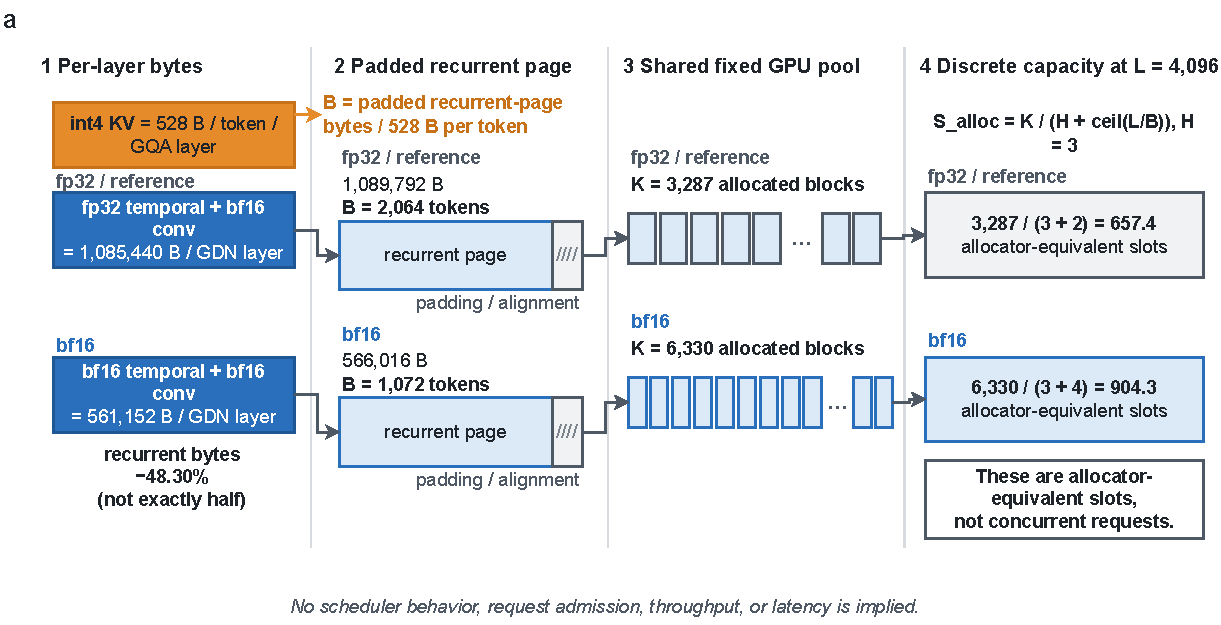
\includegraphics[width=\linewidth]{figures/drawio/fig2_discrete_allocator.pdf}
\end{minipage}\hfill
\begin{minipage}[t]{0.295\textwidth}
\vspace{0pt}
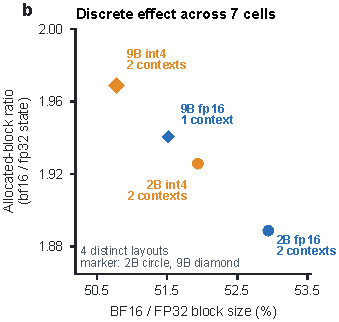
\includegraphics[width=\linewidth]{figures/vector_redesign/fig5_block_granularity.pdf}
\end{minipage}
\caption{\textbf{Byte-to-page-to-block allocation.}
(a) Verified 2B/int4/4K worked example. The recurrent-page bytes and 528-byte
int4 per-token cost determine attention block size; padding and integer block
counts then determine allocator-equivalent slots. The 657.4 and 904.3 values
are not concurrent requests. (b) Four distinct discrete layouts cover the
seven fixed-utilization cells; marker area records whether one or two context
lengths share the layout.}
\label{fig:blocks}
\end{figure*}

\begin{figure*}[!t]
\centering
\begin{minipage}[t]{0.585\textwidth}
\vspace{0pt}
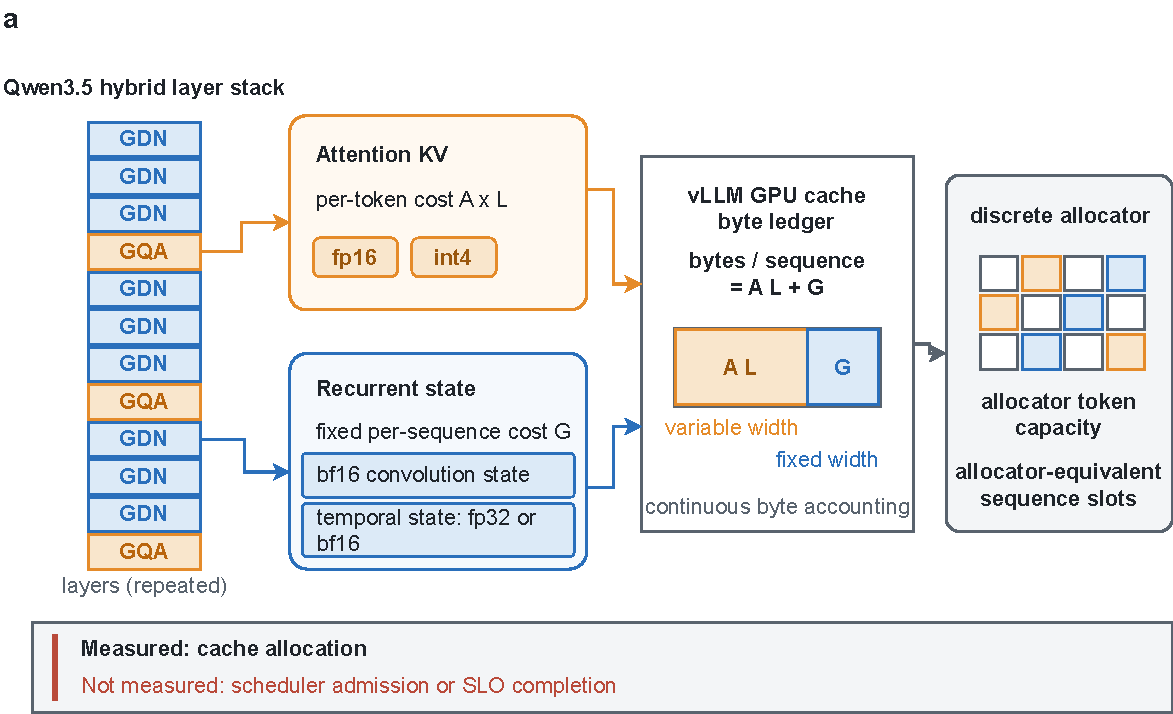
\includegraphics[width=\linewidth]{figures/drawio/fig1_hybrid_allocator.pdf}
\end{minipage}\hfill
\begin{minipage}[t]{0.385\textwidth}
\vspace{0pt}
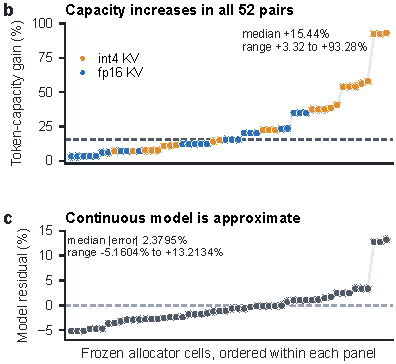
\includegraphics[width=\linewidth]{figures/vector_redesign/fig1_capacity.pdf}
\end{minipage}
\caption{\textbf{From hybrid memory to measured allocator capacity.}
(a) GQA layers contribute per-token attention KV, while GDN layers contribute
fixed recurrent state; both enter one GPU cache byte ledger before discrete
allocation. The diagram explicitly separates measured cache allocation from
unmeasured scheduler admission and SLO completion. (b) All 52 paired cells
increase allocator token capacity under bf16 state. (c) The continuous model
has mixed-sign approximation residuals and is neither a lower nor upper bound.}
\label{fig:capacity}
\end{figure*}

\section{Allocator and Decision Models}
\label{sec:model}

Let $L$ be context length, $A$ the per-token attention-KV bytes, $G$ the
fixed recurrent-state bytes per sequence, and $M$ the available cache bytes.
The continuous approximation is
\begin{equation}
  \widetilde{S}(L)=\frac{M}{A L+G}, \qquad
  \widetilde{T}(L)=L\widetilde{S}(L).
  \label{eq:continuous}
\end{equation}
Here $\widetilde{S}$ is an idealized sequence-slot count. It is not scheduler
admission. The predicted state ratio is
\begin{equation}
  r_{\mathrm{state}}(L)=
  \frac{A L+G_{\mathrm{fp32}}}{A L+G_{\mathrm{bf16}}}.
  \label{eq:rstate}
\end{equation}
The ratio decreases as $L$ grows because the attention term becomes dominant.

The engine reports a discrete capacity. Let $K$ be the allocated GPU-block
count, $H$ the number of recurrent cache groups, and $B$ the attention block
size in tokens. For this hybrid layout,
\begin{equation}
  \begin{aligned}
  S_{\mathrm{alloc}}(L) &= \frac{K}{H+\lceil L/B\rceil},\\
  T_{\mathrm{alloc}}(L) &=
    \left\lfloor L S_{\mathrm{alloc}}(L)\right\rfloor.
  \end{aligned}
  \label{eq:discrete}
\end{equation}
This equation reconstructs the reported token capacities. The Supplementary
Material provides the full parameter and padding derivation.

For deployment stratum $x$ and precision candidate $q$, the offline selector
uses
\begin{equation}
q^*(x)=\arg\max_{q\in\mathcal{F}(x)}
\underline{\mathrm{Goodput}}(q,x).
\label{eq:selector}
\end{equation}
The feasible set requires exact profile matches. It checks a quality lower
bound, latency upper bounds, cache bytes, and
$S_{\mathrm{alloc}}\ge S_{\min}$. Missing or ambiguous rows fail closed.
The selector never labels $S_{\mathrm{alloc}}$ as operational concurrency.

\section{Evaluation}
\label{sec:setup}

\textbf{Platform and allocator runs.}
We evaluate Qwen3.5-2B and 9B on one RTX 5090 with 32 GB memory. The frozen
vLLM worktrees are identified by commits \texttt{55f4768} and
\texttt{e2fa285}. The formal allocator grid crosses model, KV data type,
state data type, context length, and memory utilization. Two temporal runs
each complete 112 cells, including 52 fp32/bf16 core pairs. Allocator cells
are deterministic for a frozen build and configuration; the second attempt
checks temporal reproducibility rather than statistical replication.

\textbf{Quality and statistical units.}
The GSM8K protocol uses greedy no-think decoding and samples 200 items without
replacement for each of nine dataset seeds~\cite{gsm8k}. The same seed selects
the same ordered items for every precision candidate. The 1,800 seed-item
draws contain 1,017 unique items; pairwise seed overlap ranges from 19 to 39.
We fit an intercept-only paired contrast with two-way CR1 clustering by item
and dataset seed. Confidence intervals and nominal two-sided $p$ values use a
Student-$t$ reference with 8 degrees of freedom. A 20,000-replicate bootstrap
over unique items provides an equal-item-weight sensitivity analysis. The
nine seed summaries are descriptive, not iid replicates. This CPU reanalysis
uses Python 3.13.5, NumPy 2.1.3, SciPy 1.15.3, and statsmodels 0.14.4.

Perplexity uses a chunk-level C4/PG19 harness with three dataset seeds. RULER
uses five preregistered model-task-length cells, 20 samples per cell, and three
dataset seeds~\cite{ruler}. Exact zero RULER differences are reported as
observed equality, not equivalence.

\textbf{Selector and serving evidence.}
The selector profile contains four candidates: full, KV-only, state-only, and
joint. Each candidate stores physical cache bytes, allocator-equivalent slots,
serving bounds, and dependence-aware GSM8K intervals. We replay four frozen
requests without changing their thresholds after observing the reanalysis.

Serving uses Random60 and ShareGPT300 workloads~\cite{sharegpt}, three seed and
trace repeats, Poisson arrivals, and fixed measurement windows. A request is
good only if it completes and satisfies the specified time-to-first-token
(TTFT) and time-per-output-token (TPOT) limits. SLO-goodput is the number of
good requests divided by measurement duration. Failed requests remain in the
denominator. A second run uses the same host, contracts, and seeds, so we call
it a temporal rerun.

\section{Results}
\label{sec:results}

\subsection{Allocator capacity}
\label{sec:capacity}

\begin{table}[t]
\centering
\scriptsize
\caption{\textbf{Fixed-utilization allocator slice.} Token columns are total
allocator token capacity. Gap is
$(r_{\mathrm{measured}}-r_{\mathrm{model}})/r_{\mathrm{model}}$. The
9B/fp16/16K cell was not probed in the frozen 0.85 fp16 attempt; it is not
silently imputed.}
\label{tab:capacity}
\setlength{\tabcolsep}{3.1pt}
\begin{tabular}{llrrrl}
\toprule
KV & Cell & fp32 total & bf16 total & ratio & gap\\
\midrule
int4 & 2B/4K  & 2,692,710 & 3,703,954 & 1.3755 & $-2.37\%$\\
int4 & 2B/16K & 4,895,837 & 5,458,458 & 1.1149 & $-3.24\%$\\
int4 & 9B/4K  &   315,392 &   443,538 & 1.4063 & $-0.19\%$\\
int4 & 9B/16K &   573,440 &   653,635 & 1.1398 & $-1.07\%$\\
fp16 & 2B/4K  & 1,199,383 & 1,384,448 & 1.1543 & $-0.16\%$\\
fp16 & 2B/16K & 1,552,143 & 1,661,337 & 1.0704 & $+2.46\%$\\
fp16 & 9B/4K  &   144,104 &   161,899 & 1.1235 & $-2.83\%$\\
\bottomrule
\end{tabular}
\end{table}

Across the formal 52-pair matrix, every bf16-state cell has higher allocator
token capacity than its fp32-state pair. The median gain is 15.44\%, and the
range is 3.32--93.28\%. The largest gains occur in short-context cells where
fixed state dominates. The temporal rerun reproduces all 112 cells within the
frozen token tolerance; the largest per-cell difference is 1.42\%.

The corrected continuous model has 2.3795\% median absolute residual. Signed
residuals range from $-5.1604\%$ to $+13.2134\%$. Their mixed signs rule out a
lower-bound or upper-bound interpretation. Figure~\ref{fig:capacity} compares
the model with the fixed-utilization slice.

The byte correction matters. Each GDN layer contains a 36,864-byte bf16
convolution state plus a temporal state. Changing only the temporal state from
fp32 to bf16 reduces per-layer bytes from 1,085,440 to 561,152, or 48.30\%.
It does not halve the complete GDN state. Figure~\ref{fig:blocks} shows how the
smaller recurrent page changes discrete block sizes and counts.

For 2B/int4/4K, fp32 uses $K=3287$, $B=2064$, and $H=3$.
Equation~\eqref{eq:discrete} gives $3287/(3+2)=657.4$ slots and 2,692,710
tokens. Bf16 uses $K=6330$ and $B=1072$, giving $6330/(3+4)=904.3$ slots and
3,703,954 tokens. The difference is 246.9 allocator-equivalent slots. We have
not shown that a scheduler admits or completes that many simultaneous 4K
requests under an SLO.

\subsection{Quality evidence}
\label{sec:quality}

Figure~\ref{fig:gsm8k} reports the corrected GSM8K analysis. At 2B,
state-only changes accuracy by $-1.000$ percentage point
(95\% CI $[-2.044,+0.044]$, nominal $p=0.0582$). The equal-item sensitivity
estimate is $-0.778$ points ($[-1.958,+0.410]$), with 29 gain items and 37 loss
items. Int4 KV changes accuracy by $-2.722$ points
($[-5.275,-0.169]$, nominal $p=0.0394$). Joint precision changes it by
$-1.556$ points ($[-4.447,+1.336]$, nominal $p=0.2499$). The joint-minus-KV
contrast is $+1.167$ points ($[-0.987,+3.321]$). At 9B, state-only changes
accuracy by $+0.333$ points ($[-0.138,+0.804]$, nominal $p=0.1414$).

These are candidate-specific guardrail intervals, not a multiplicity-adjusted
discovery family. Only the 2B int4-KV nominal interval excludes zero. We do not
describe state-only or joint precision as quality preserving, beneficial, or
non-inferior.

\begin{figure}[t]
\centering
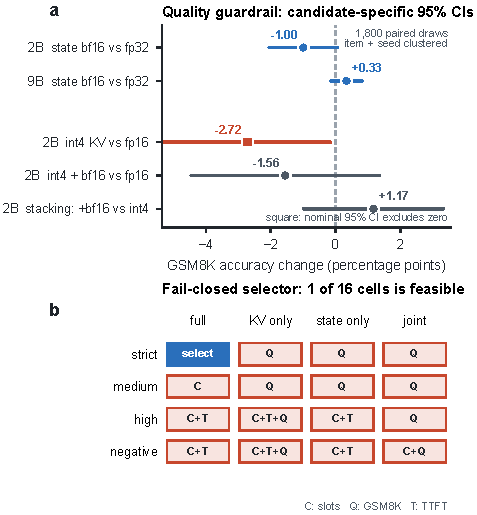
\includegraphics[width=\linewidth]{figures/vector_redesign/fig2_gsm8k.pdf}
\caption{\textbf{Quality evidence and selector consequence.} (a) The primary
GSM8K analysis uses
1,800 paired seed-item draws, 1,017 item clusters, nine dataset-seed clusters,
two-way CR1 covariance, and a Student-$t$ reference with 8 df. Squares mark a
nominal 95\% interval excluding zero; color is redundant. No multiplicity
adjustment is applied across the displayed contrasts. (b) Complete frozen
selector audit. C, Q, and T denote rejection by allocator slots, GSM8K quality,
and TTFT, respectively. Only strict/full is feasible and selected.}
\label{fig:gsm8k}
\end{figure}

On C4, PPL changes by $-0.0029$, with a 95\% CI from $-0.0129$ to
$+0.0072$. On PG19, it changes by $+0.0065$, with a CI from $-0.0447$ to
$+0.0578$. Both intervals include zero and do not establish equivalence. The
harness also rounds state at chunk boundaries, so it is supporting evidence
only. In five no-think RULER cells, both temporal runs observe identical fp32
and bf16 outputs across three seeds. The resulting zero-width descriptive
intervals are observed equality, not population certainty
(Figure~\ref{fig:ruler}).

\begin{figure}[t]
\centering
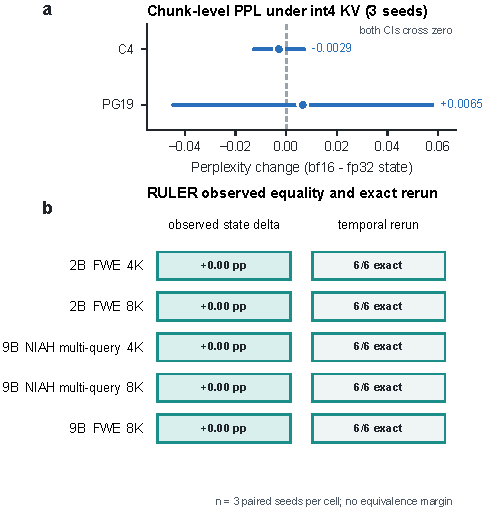
\includegraphics[width=\linewidth]{figures/vector_redesign/fig3_ppl_ruler.pdf}
\caption{\textbf{PPL and RULER boundaries.} (a) Chunk-level PPL contrasts for
C4 and PG19. (b) Five no-think RULER cells have exact observed equality; each
cell also has 6/6 exact temporal matches across three seeds and two allocations
(30/30 total). Zero-width descriptive intervals and exact reruns are not an
equivalence or non-inferiority test.}
\label{fig:ruler}
\end{figure}

An exploratory 18-layer sensitivity screen produces two raw C4 intervals with
$p<0.05$, but neither survives Bonferroni or Benjamini--Hochberg correction.
This result does not show that whole-state precision is optimal. It only
provides no corrected evidence for a layer exception in this screen. The
Supplementary Material reports the panel and the chunk-size ablation.

\subsection{Corrected selector audit}
\label{sec:controller}

Table~\ref{tab:selector-audit} replays the four frozen requests after replacing
seed-iid quality bounds with the clustered intervals above. The strict request
requires 250 allocator-equivalent slots and a $-1.0$ point GSM8K floor. Full
precision is its only feasible candidate and has a 29.483 req/s SLO-goodput
lower bound.

The medium request has no feasible candidate. Full precision provides only
269.9 slots against a requirement of 300. State-only provides 311.6 slots, but
its quality lower bound is $-2.044$ points against a $-2.0$ point floor. KV-only
and joint also violate quality. For the high request, joint provides enough
slots but misses the $-4.0$ point quality floor. The negative control requires
900 slots, which no candidate provides. We did not relax any threshold after
seeing these outcomes.

\begin{table*}[t]
\centering
\caption{Frozen selector audit after dependence-aware GSM8K reanalysis. Quality values are percentage-point differences from full precision. Slots are allocator-equivalent sequence slots, not demonstrated scheduler concurrency.}
\label{tab:selector-audit}
\small
\setlength{\tabcolsep}{3.5pt}
\begin{tabular}{llrrrrl}
\toprule
Budget & Candidate & Required slots & Quality floor & Quality 95\% CI & Goodput LCB & Outcome \\
 & & & (pp) & (pp) & (req/s) & \\
\midrule
strict & full & 250 & -1.0 & [+0.00, +0.00] & 29.483 & \textbf{selected} \\
 & kv\_only & 250 & -1.0 & [-5.28, -0.17] & 29.358 & reject: quality \\
 & state\_only & 250 & -1.0 & [-2.04, +0.04] & 29.487 & reject: quality \\
 & joint & 250 & -1.0 & [-4.45, +1.34] & 29.357 & reject: quality \\
\addlinespace[2pt]
medium & full & 300 & -2.0 & [+0.00, +0.00] & 29.483 & reject: slots \\
 & kv\_only & 300 & -2.0 & [-5.28, -0.17] & 29.358 & reject: quality \\
 & state\_only & 300 & -2.0 & [-2.04, +0.04] & 29.487 & reject: quality \\
 & joint & 300 & -2.0 & [-4.45, +1.34] & 29.357 & reject: quality \\
\addlinespace[2pt]
high & full & 700 & -4.0 & [+0.00, +0.00] & 7.948 & reject: slots, TTFT \\
 & kv\_only & 700 & -4.0 & [-5.28, -0.17] & 32.137 & reject: slots, TTFT, quality \\
 & state\_only & 700 & -4.0 & [-2.04, +0.04] & 15.356 & reject: slots, TTFT \\
 & joint & 700 & -4.0 & [-4.45, +1.34] & 37.624 & reject: quality \\
\addlinespace[2pt]
negative & full & 900 & -4.0 & [+0.00, +0.00] & 7.948 & reject: slots, TTFT \\
 & kv\_only & 900 & -4.0 & [-5.28, -0.17] & 32.137 & reject: slots, TTFT, quality \\
 & state\_only & 900 & -4.0 & [-2.04, +0.04] & 15.356 & reject: slots, TTFT \\
 & joint & 900 & -4.0 & [-4.45, +1.34] & 37.624 & reject: slots, quality \\
\bottomrule
\end{tabular}
\end{table*}


This audit invalidates the earlier three-mapping narrative. It demonstrates
fail-closed constraint evaluation and complete rejection traces. It does not
demonstrate an optimal online policy, held-out regret, or a serving advantage.

\subsection{Serving boundary}
\label{sec:serving}

Figure~\ref{fig:serving} shows the formal run and temporal rerun for Random60
and ShareGPT300. None of the 60 cellwise comparisons survives Benjamini--
Hochberg false-discovery-rate control. Random60 overload cells have consistent
directions across runs, while ShareGPT directions do not. We therefore do not
claim a workload-general goodput effect.

The controlled mechanism matrix completes 18 cells in each run. Throughput is
within 10\% in 18/18 temporal comparisons, TTFT in 10/18, and TPOT in 17/18.
None of nine contrast tests survives Holm correction. The broader
four-configuration matrix completes 144/144 cells per run, yet fails its
primary stability gate: 183/720 continuous-goodput comparisons exceed the
10\% tolerance. Binary SLO labels are more stable, but they do not override
the failed primary endpoint.

\begin{figure*}[t]
\centering
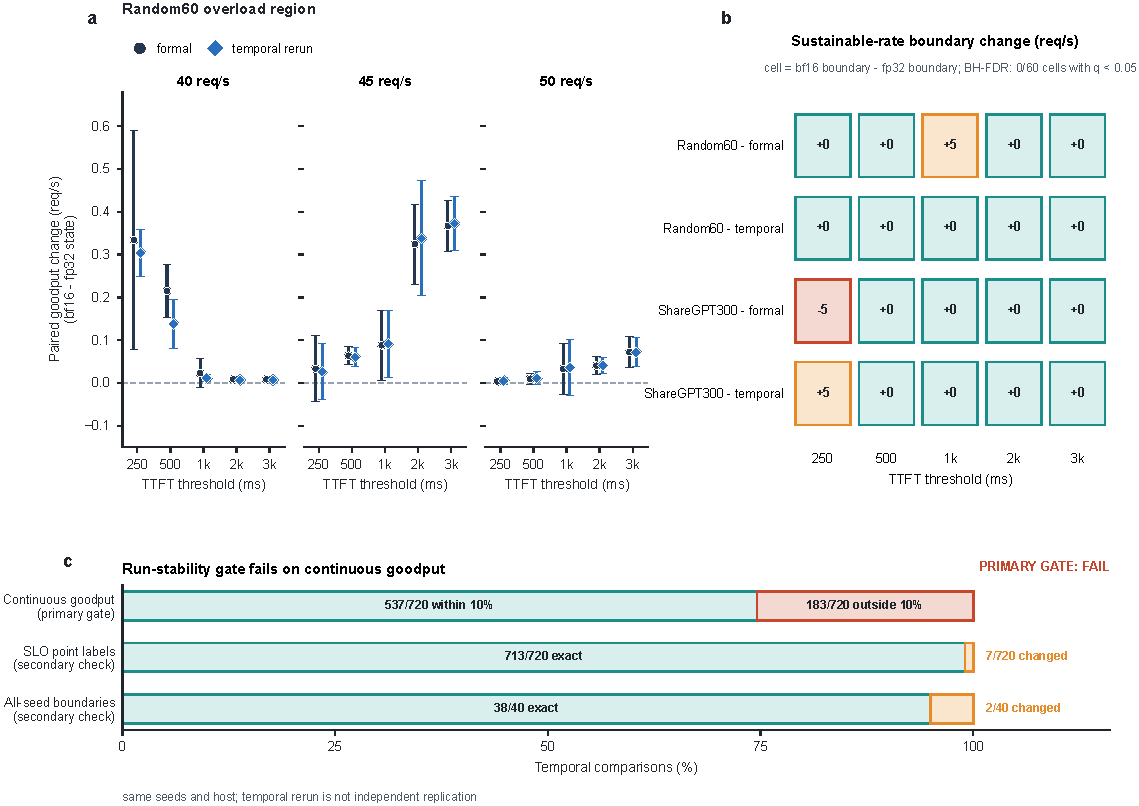
\includegraphics[width=\textwidth]{figures/vector_redesign/fig4_serving.pdf}
\caption{\textbf{Serving run-stability evidence.} (a) Random60 paired goodput
change in req/s for the formal run and temporal rerun. (b) Sustainable-rate
boundary changes for Random60 and ShareGPT300. The rerun uses the same host,
contracts, and seeds. None of 60 cellwise comparisons survives BH-FDR.
(c) The four-configuration temporal audit fails its predeclared continuous-
goodput gate: 183/720 comparisons exceed 10\%. Exact binary SLO labels
(713/720) do not override the failed primary endpoint.}
\label{fig:serving}
\end{figure*}

\clearpage
\balance
\section{Discussion and Limitations}
\label{sec:limits}

\textbf{Allocator capacity is not serving concurrency.}
The engine's token ceiling and Eq.~\eqref{eq:discrete} describe cache
allocation. They do not measure request admission, prefill, decode, completion,
out-of-memory boundaries, or SLO success at the reported slot count. This is
the central scope boundary of the paper.

\textbf{The continuous model is approximate.}
It omits discrete attention blocks, recurrent-page padding, and layout
alignment. Correct byte accounting reduces state by 48.30\%, not 50\%. The
observed residual range has both signs, so extrapolation outside measured
strata requires a fresh probe.

\textbf{Quality inference remains scoped.}
Two-way clustering addresses repeated items and shared dataset seeds, but
repeated greedy evaluations still show inconsistent outcomes for some items.
The 2B baseline has 30 such repeated items and state-only has 27. The item
bootstrap targets a different equal-item estimand and gives a similar state
estimate, but it does not explain this variability. The contrasts are also
not adjusted as one discovery family.

\textbf{The selector is an audited, fail-closed lookup policy.}
It uses cold-start, exact-stratum profiles without interpolation, oracle
comparison, or measured switching overhead. Because cache precision may alter
outputs used for agent planning or tool selection, a configuration is admitted
only when its capacity target, quality bounds, and SLO evidence all pass;
missing evidence rejects it. We do not evaluate prompt injection, data leakage, cache isolation,
adversarial robustness, policy compliance, or agent safety.

\textbf{System and hardware coverage is narrow.}
All measurements use Qwen3.5-2B/9B, one RTX 5090, and one vLLM lineage. Tensor
parallelism, prefix caching, offloading, other hybrid architectures, and other
accelerators can change both terms and rounding. The PPL harness is not a
per-token kernel equivalence test, and RULER has only three dataset seeds.

\textbf{Artifact status is local.}
The current submission has no public artifact URL. Reproducibility claims
refer to repository-local JSON, CSV, scripts, and SHA-256 sidecars. The figure
verifier pins 16 source hashes, checks all 52 paired capacity rows, and fails
on numeric drift. Public release and independent-host validation remain future
work.

\section{Conclusion}
\label{sec:conclusion}

Hybrid LLM cache accounting must include both per-token attention KV and fixed
recurrent state. In the measured Qwen3.5/vLLM matrix, bf16 temporal state raises
allocator token capacity in all 52 pairs, with a 15.44\% median increase. The
effect is strongest at short contexts, but the continuous model retains
material, mixed-sign residuals.

The dependence-aware audit leaves only the strict request feasible at full
precision, while the serving matrix provides no stable end-to-end benefit. For
agent deployments, cache precision is therefore a safety-relevant configuration:
capacity, quality bounds, and SLO evidence must all pass, and missing evidence
must fail closed.
This work does not establish agentic or adversarial safety, including defenses
against prompt injection, data leakage, cache-isolation failures, adversarial
behavior, or policy violations.

\bibliographystyle{IEEEtran}
\bibliography{main}

\end{document}
